\documentclass[letter,twocolumn]{article}

\usepackage{geometry}
\geometry{
		total={7.5in,10in},
	}



\usepackage{graphics}
\usepackage{graphicx} % For including and formatting image files
\usepackage{multirow}
\usepackage{longtable}
\usepackage{epsfig}
\usepackage{epstopdf}

\usepackage{amsmath, mathrsfs, dsfont}
\usepackage{amssymb}
\usepackage{amsfonts}
\usepackage{amsbsy}
\usepackage{bm}


\usepackage{cite}
\usepackage{verbatim}

\usepackage{amscd}
\usepackage{color}
\definecolor{lgray}{gray}{0.6}
\usepackage{rotating}


%\usepackage[font=footnotesize]{caption}
%\usepackage[caption=false,font=footnotesize]{subfig}
\usepackage[font=footnotesize]{subcaption}

\usepackage{mathptmx}
\usepackage[11pt]{moresize}
\usepackage{flushend}
\usepackage[stable]{footmisc}

\usepackage{algorithmicx}
\usepackage{algorithm}
\usepackage{algpascal}
\usepackage{float}
\usepackage{algc}
\usepackage{algcompatible}
\usepackage{algpseudocode}

\renewcommand{\algorithmicrequire}{\textbf{Input:}}  % Use Input in the format of Algorithm  
\renewcommand{\algorithmicensure}{\textbf{Output:}} % Use Output in the format of Algorithm  
\usepackage[vcentermath]{youngtab} % For typesetting Young Tableaux
\usepackage{url}
%\usepackage{breakurl}   
            

%-----------------------------------------%
% Define custom symbols
\newcommand{\BoldA}				{ \mathbf{A} }
\newcommand{\Bolda}				{ \mathbf{a} }
\newcommand{\BoldB}				{ \mathbf{B} }
\newcommand{\Boldb}				{ \mathbf{b} }
\newcommand{\BoldC}				{ \mathbf{C} }
\newcommand{\Boldc}				{ \mathbf{c} }
\newcommand{\BoldD}				{ \mathbf{D} }
\newcommand{\Boldd}				{ \mathbf{d} }
\newcommand{\BoldE}				{ \mathbf{E} }
\newcommand{\Bolde}				{ \mathbf{e} }
\newcommand{\BoldF}				{ \mathbf{F} }
\newcommand{\Boldf}				{ \mathbf{f} }
\newcommand{\BoldG}				{ \mathbf{G} }
\newcommand{\g}					{ \mathbf{g} }
\newcommand{\BoldH}				{ \mathbf{H} }
\newcommand{\Boldh}				{ \mathbf{h} }
\newcommand{\BoldI}				{ \mathbf{I} }
\newcommand{\I}					{ \mathbf{I} }
\newcommand{\BoldJ}				{ \mathbf{J} }
\newcommand{\BoldK}				{ \mathbf{K} }
\newcommand{\Boldk}				{ \mathbf{k} }
\newcommand{\BoldM}				{ \mathbf{M} }
\newcommand{\BoldN}				{ \mathbf{N} }
\newcommand{\Boldn}				{ \mathbf{n} }
\newcommand{\BoldO}				{ \mathbf{O} }
\newcommand{\BoldP}				{ \mathbf{P} }
\newcommand{\Boldp}				{ \mathbf{p} }
\newcommand{\BoldQ}				{ \mathbf{Q} }
\newcommand{\Boldq}				{ \mathbf{q} }
\newcommand{\BoldR}				{ \mathbf{R} }
\newcommand{\R}					{ \mathbf{R} }
\newcommand{\Boldr}				{ \mathbf{r} }
\newcommand{\Bolds}				{ \mathbf{s} }
\newcommand{\BoldS}				{ \mathbf{S} }
\newcommand{\BoldT}				{ \mathbf{T} }
\newcommand{\BoldU}				{ \mathbf{U} }
\newcommand{\Boldu}				{ \mathbf{u} }
\newcommand{\BoldV}				{ \mathbf{V} }
\newcommand{\Boldv}				{ \mathbf{v} }
\newcommand{\Boldw}				{ \mathbf{w} }
\newcommand{\BoldW}				{ \mathbf{W} }
\newcommand{\BoldX}				{ \mathbf{X} }
\newcommand{\Boldx}				{ \mathbf{x} }
\newcommand{\BoldY}				{ \mathbf{Y} }
\newcommand{\Boldy}				{ \mathbf{y} }
\newcommand{\BoldZ}				{ \mathbf{Z} }
\newcommand{\Boldz}				{ \mathbf{z} }


\newcommand{\0}					{ \boldsymbol{0} }
\newcommand{\1}					{ \boldsymbol{1} }

\newcommand{\dtheta}			{ \delta\boldsymbol{\theta} }
\newcommand{\noiseg}			{ \mathbf{n}_{g} }
\newcommand{\noisewg}			{ \mathbf{n}_{{\omega}g} }
\newcommand{\noisea}			{ \mathbf{n}_{a} }
\newcommand{\noisewa}			{ \mathbf{n}_{{\omega}a} }
\newcommand{\Boldomega}			{ \boldsymbol{\omega} }
\newcommand{\Boldnu}			{ \boldsymbol{\nu} }
\newcommand{\BoldGamma}			{ \boldsymbol{\Gamma} }
\newcommand{\Boldgamma}			{ \boldsymbol{\gamma} }
\newcommand{\Boldkappa}			{ \boldsymbol{\kappa} }
\newcommand{\BoldPhi}			{ \boldsymbol{\Phi} }
\newcommand{\Boldphi}			{ \boldsymbol{\phi} }
\newcommand{\Boldpi}			{ \boldsymbol{\pi} }
\newcommand{\Boldrho}			{ \boldsymbol{\rho} }
\newcommand{\Boldell}			{ \boldsymbol{\ell} }
%\newcommand{\0}					{ \boldsymbol{0} }
\newcommand{\Bolddelta}			{ \boldsymbol{\delta} }
\newcommand{\BoldDelta}			{ \boldsymbol{\Delta} }
\newcommand{\BoldTheta}			{ \boldsymbol{\Theta} }
\newcommand{\Boldtheta}			{ \boldsymbol{\theta} }
\newcommand{\BoldSigma}			{ \boldsymbol{\Sigma} }
\newcommand{\Boldsigma}			{ \boldsymbol{\sigma} }
\newcommand{\Boldeps}			{ \boldsymbol{\epsilon} }
\newcommand{\Boldmu}			{ \boldsymbol{\mu} }
\newcommand{\Boldeta}			{ \boldsymbol{\eta} }
\newcommand{\Boldzeta}			{ \boldsymbol{\zeta} }
\newcommand{\Boldlambda}		{ \boldsymbol{\lambda} }
\newcommand{\BoldLambda}		{ \boldsymbol{\Lambda} }
\newcommand{\Boldchi}			{ \boldsymbol{\chi} }

\newcommand{\E}					{\mathrm{E}}
\newcommand{\Var}				{\mathrm{Var}}
\newcommand{\Cov}				{\mathrm{Cov}}
\newcommand\norm[1]{\lVert#1\rVert}

\newcommand\T{\rule{0pt}{2.6ex}}       % Top strut
\newcommand\B{\rule[-1.2ex]{0pt}{0pt}} % Bottom strut

\newcounter{inlineenum}
\renewcommand{\theinlineenum}{\alph{inlineenum}}
\newenvironment{inlineenum}
{\unskip\ignorespaces\setcounter{inlineenum}{0}%
	\renewcommand{\item}{\refstepcounter{inlineenum}{\textit{\theinlineenum})~}}}

\newcommand{\icol}[1]{% inline column vector
	\left(\begin{matrix}#1\end{matrix}\right)%
}
\newcommand{\irow}[1]{% inline row vector
	\begin{matrix}(#1)\end{matrix}%
}

%-----------------------------------------%
% Define custom operators
\DeclareMathOperator*{\argmin}{\emph{arg\,min}}
\DeclareMathAlphabet{\mathcal}{OMS}{cmsy}{m}{n}

%-----------------------------------------%
% Define custom commands
%\newcommand{\or}{\bf or}
%\newcommand{\and}{\bf and}
\newtheorem{Theorem}{Theorem}[section]
\newtheorem{Proposition}[Theorem]{Proposition}
\newtheorem{Lemma}[Theorem]{Lemma}
\newtheorem{Corollary}[Theorem]{Corollary}
\newtheorem{Remark}[Theorem]{\textbf{Remark}}
	\newcommand{\brmrk}[1]{\begin{remark} \label{#1} }
	\newcommand{\ermrk}{ \hfill $\bigtriangleup$    \end{remark} \vspace{1mm} }
\newtheorem{Definition}[Theorem]{Definition}
\newtheorem{Example}[Theorem]{Example}
\newtheorem{Conjecture}[Theorem]{Conjecture}
\newtheorem{Problem}[Theorem]{Problem}
\newtheorem{Algorithm}[Theorem]{Algorithm}
\newtheorem{CardGame}[Theorem]{Card Game}
\newtheorem{Strategy}[Theorem]{Strategy}
\newtheorem{Question}[Theorem]{Question}
\newtheorem{exercise}{Exercise}[section]
\newcommand{\boex}[1]{\begin{example} \label{#1} --- \rm}
	\newcommand{\eoex}{ \hfill $\bigtriangleup$    \end{example} \vspace{1mm} }
\newtheorem{example}{Example}[section]
\newcommand{\bohw}[1]{\begin{exercise} \label{#1} -- \rm}
	\newcommand{\eohw}{ \hfill    \end{exercise} \vspace{1mm} }
\newtheorem{assumption}{Assumption}[section]
	\newcommand{\boass}[1]{\begin{assumption} \label{#1} -- \rm}
	\newcommand{\eoass}{ \hfill    \end{assumption} \vspace{1mm} }

\newcommand{\todo}[1]{\footnote{\color{green}TO DO: {#1}}}

\newcommand{\tstamp}{\today}
%\usepackage{fancyhdr}
%\pagestyle{fancy}
%\headheight 35pt

%\rhead{\tstamp}
%\chead{Middle top}
%\lhead{Left top}
%\rfoot{p. \thepage}
%\cfoot{}
%\lfoot{Copyright \textcopyright 2019, University of California, Riverside. All Rights reserved.}

\renewcommand{\baselinestretch}{1.0}

\setcounter{secnumdepth}{3}
\setcounter{tocdepth}{2}

\newcommand{\black}{\color{black}}
\newcommand{\blue}{\color{blue}}
\newcommand{\red}{\color{red}}
\newcommand{\green}{\color{green}}
\newcommand{\magenta}{\color{magenta}}
\newcommand{\cyan}{\color{cyan}}
\newcommand{\orange}{\color{orange}}
\definecolor{brinkpink}{rgb}{1.00, 0.33, 0.64}
\newcommand{\pink}{\color{brinkpink}}

%\newcommand{\black}{\color{black}}
%\newcommand{\blue}{\color{black}}
%\newcommand{\red}{\color{black}}
%\newcommand{\green}{\color{black}}
%\newcommand{\magenta}{\color{black}}

\makeatletter
\newenvironment{breakablealgorithm}
{% \begin{breakablealgorithm}
	\begin{center}
		\refstepcounter{algorithm}% New algorithm
		\hrule height.8pt depth0pt \kern2pt% \@fs@pre for \@fs@ruled
		\renewcommand{\caption}[2][\relax]{% Make a new \caption
			{\raggedright\textbf{\ALG@name~\thealgorithm} ##2\par}%
			\ifx\relax##1\relax % #1 is \relax
			\addcontentsline{loa}{algorithm}{\protect\numberline{\thealgorithm}##2}%
			\else % #1 is not \relax
			\addcontentsline{loa}{algorithm}{\protect\numberline{\thealgorithm}##1}%
			\fi
			\kern2pt\hrule\kern2pt
		}
	}{% \end{breakablealgorithm}
		\kern2pt\hrule\relax% \@fs@post for \@fs@ruled
	\end{center}
}
\makeatother







 

\begin{document}
	\title{ASD to State-Space Recipe Book}
\author{Jay~A.~Farrell}
\maketitle

\begin{abstract}
This article walks through the process for extracting first-order state-space (Gauss-Markov) models corresponding to an ASD plot for a range of delays.
This article skips all derivations, many of which are presented or pointed to in \cite{CSM_IMU}.

This methods herein apply to both gyros and accelerometers. 
To be generic, the article will use the terminology of phase and frequency. 
The term {\em frequency} refers to the either the IMU angular rate or specific force measurement.
The term {\em phase} refers to the integral of frequency, which for an IMU refers to attitude or velocity. 

Given values of $N$, $B$, $T_p$, and $F_s$, the script ASD\_to\_GaussMarkovFirstOrder.py implements all the computations that are presented herein in a \blue blue \black font.  
\end{abstract}

\section{ASD Graph to State-Space Model}

This section assumes that an ASD plot is available. 
Samples of an example ASD curve are shown as blue dots in the figures herein.
\begin{enumerate}
	\item Find the portion of the ASD graph that has a slope of -1/2. Draw a tangent line, and define phase random walk parameter $N$ as the value of this ASD tangent line where it crosses the vertical line at $\tau = 1$. See the example orange lines in Fig. \ref{fig:ASD_plot_N_B}.
	
	\begin{figure}[htb]
		\centering
		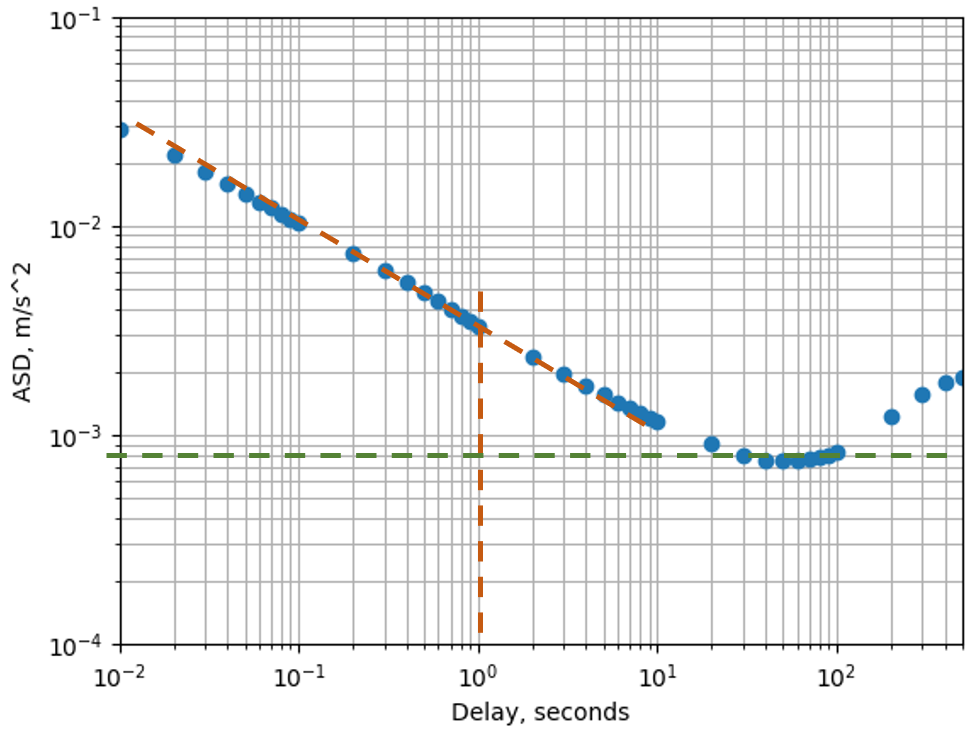
\includegraphics[trim=0in 0in 0in 0.1in, clip, width=0.8\columnwidth]{figure/ASD_plot_N_B}
		\caption{Allan Standard Deviation Plot marked for estimation of $N$ and $B$. 
			The slanted orange line with slope -1/2 intersects the vertical line at $\tau=1$ for $N$ = 3.3e-3 m/s/s/rtHz. The horizontal dashed green line defines $B=8.0 e-3$ m/s/s. }
		\label{fig:ASD_plot_N_B}
	\end{figure}
	
	\item The continuous-time phase random walk power spectral density is \blue $S_n=N^2$. \black
	\item The discrete-time phase random walk covariance is \blue $Q_\nu = S_n \, F_s$. \black
	\item The values of $B$ and $T_p$ are selected together. 
	\begin{itemize}
		\item 	By definition $B$ is the value of the ASD plot at which its slope is zero. For many inexpensive IMU's this flat section may not exist or may be difficult to select due to the noisiness of the ASD plot. 
		The ASD plot in Fig. \ref{fig:ASD_plot_N_B} is very clean and a reasonable value of $B$ can be read off. 
		\item There is not finite-dimensional state space-model that can exactly reproduce the bias instabiility. See \cite{CSM_IMU}.
		
		\item This example selects the first-order model 
		\begin{align} \label{eqn:GM}
			\dot{b}(t) = -\mu \, b(t) + \omega(t)
		\end{align}
		to approximate the bias instability portion of the ASD plot. 
		The shape of the ASD plot corresponding to this model is sketched as the green asymptotes and black curve in Fig. \ref{fig:ASD_plot_N_B}. 
		It has a peak at $T_p$ and and the asymptotes have slope $\pm 1/2$;
		therefore, for delays near, but smaller that $T_p$, the parameters $B$ and $T_p$ can be selected to produce a flat region with the desired height. 
		Given values for $B$ and $T_p$, the script computes:
		\begin{align*}
		\blue \T_b &= \blue \frac{T_p}{1.89}, \black && \mbox{a parameter for the ASD model} \\
		\blue \mu &= \blue\frac{1}{T_b} \black  && \mbox{the decay rate in eqn. \eqref{eqn:GM}} \\
		\blue S_b &= \blue\frac{B^2}{0.4365^2\,T_b} \black && \mbox{PSD of } \omega(t) \\
		\blue \bar{P}_b & = \blue\frac{S_b}{2\,\mu} \black && \mbox{steady state covariance of } b(t) 
		\end{align*}
	\end{itemize}

\end{enumerate}

\begin{figure}[tbh]
	\centering
	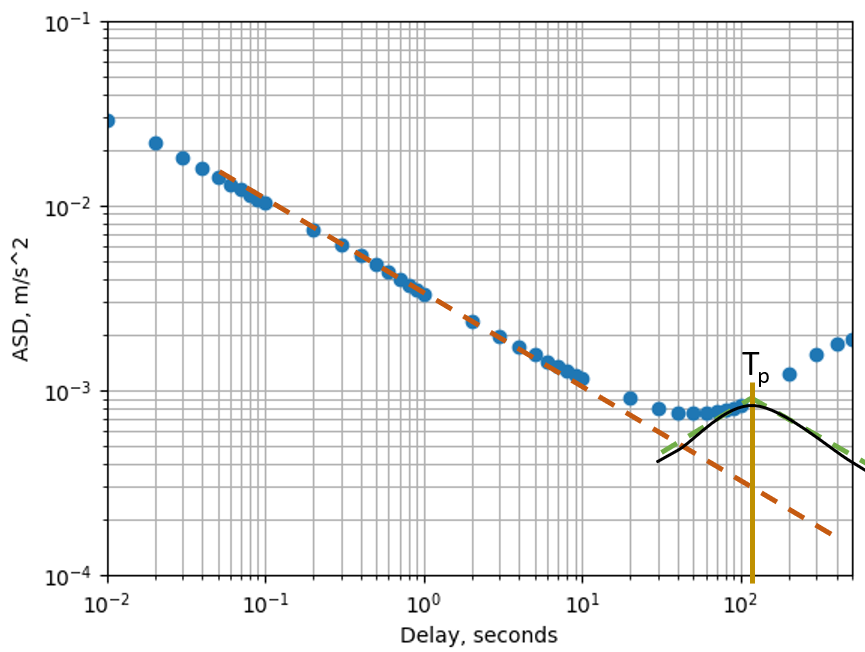
\includegraphics[trim=0in 0in 0in 0.1in, clip, width=0.8\columnwidth]{figure/ASD_plot_B_GM}
	\caption{Allan Standard Deviation Plot marked with approximations for the first-order Gauss-Markov model. }
	\label{fig:ASD_plot_B_GM}
\end{figure}

The script also provides tools to convert the continuous-time model to and equivalent discrete-time model, to simulate the model of produce sample data, and to plot the Allan standard deviation plots. The red dots in Fig. \ref{fig:ASD_plot}  show the results of this process.

\begin{figure}[tbh]
	\centering
	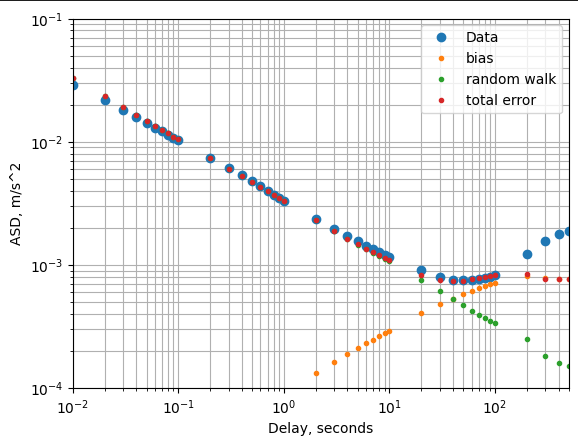
\includegraphics[trim=0in 0in 0in 0.1in, clip, width=0.9\columnwidth]{figure/ASD_plot}
	\caption{Allan Standard Deviation Plot.}
	\label{fig:ASD_plot}
\end{figure}

\vfill

\bibliographystyle{IEEEtran}
\bibliography{refs.bib}
\end{document}